\documentclass[tikz,border=10pt]{standalone}
\usetikzlibrary{positioning, arrows.meta, calc, babel}
\usepackage[utf8]{inputenc}
\usepackage[T1]{fontenc}
\usepackage{lmodern}
\usepackage[english]{babel}
\usepackage{amsmath, amssymb, bm}

\begin{document}
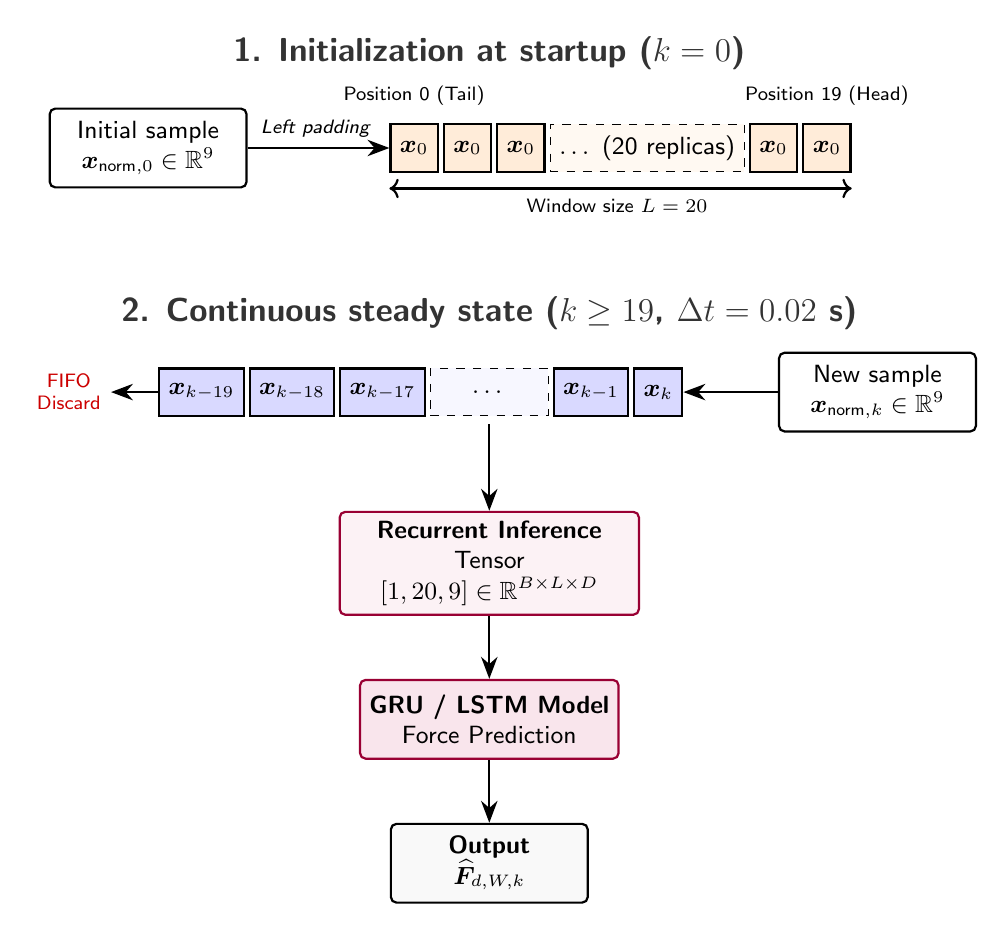
\begin{tikzpicture}[
  node distance=0.6cm and 0.8cm,
  align=center,
  font=\sffamily\small,
  % Estilos de celdas de la cola
  padcell/.style={draw, rectangle, minimum size=0.6cm, fill=orange!15, thick},
  realcell/.style={draw, rectangle, minimum size=0.6cm, fill=blue!15, thick},
  % Estilos de bloques
  box/.style={draw, rectangle, rounded corners=2pt, minimum width=2.5cm, minimum height=1.0cm, thick, fill=white},
  % Estilos de flechas
  line/.style={draw, -{Stealth[scale=1.2]}, thick}
]

  % ==========================================
  % PANEL 1: INITIALIZATION AT STARTUP (k=0)
  % ==========================================
  \node[padcell] (c0_0) at (3., 2.3) {$\bm{x}_{0}$};
  \node[padcell, right=0.05cm of c0_0] (c0_1) {$\bm{x}_{0}$};
  \node[padcell, right=0.05cm of c0_1] (c0_2) {$\bm{x}_{0}$};
  \node[draw, rectangle, dashed, minimum width=1.5cm, minimum height=0.6cm, right=0.05cm of c0_2, fill=orange!5] (c0_mid) {$\dots$ (20 replicas)};
  \node[padcell, right=0.05cm of c0_mid] (c0_18) {$\bm{x}_{0}$};
  \node[padcell, right=0.05cm of c0_18] (c0_19) {$\bm{x}_{0}$};

  % Queue labels
  \node[above=0.1cm of c0_0, font=\sffamily\scriptsize] {Position 0 (Tail)};
  \node[above=0.1cm of c0_19, font=\sffamily\scriptsize] {Position 19 (Head)};
  \draw[thick, <->] ($(c0_0.south west) + (0,-0.2)$) -- node[below, font=\sffamily\scriptsize] {Window size $L = 20$} ($(c0_19.south east) + (0,-0.2)$);

  % Initial input
  \node[box, fill=white, left=1.8cm of c0_0] (input0) {Initial sample\\$\bm{x}_{\text{norm}, 0} \in \mathbb{R}^9$};
  \draw[line] (input0.east) -- node[above, font=\sffamily\scriptsize\itshape] {Left padding} (c0_0.west);


  % ==========================================
  % PANEL 2: CONTINUOUS STEADY STATE (k >= 19)
  % ==========================================
  \node[realcell] (c1_0) at (0.3, -0.8) {$\bm{x}_{k-19}$};
  \node[realcell, right=0.05cm of c1_0] (c1_1) {$\bm{x}_{k-18}$};
  \node[realcell, right=0.05cm of c1_1] (c1_2) {$\bm{x}_{k-17}$};
  \node[draw, rectangle, dashed, minimum width=1.5cm, minimum height=0.6cm, right=0.05cm of c1_2, fill=blue!3] (c1_mid) {$\dots$};
  \node[realcell, right=0.05cm of c1_mid] (c1_18) {$\bm{x}_{k-1}$};
  \node[realcell, right=0.05cm of c1_18] (c1_19) {$\bm{x}_{k}$};

  % Current sample input
  \node[box, fill=white, right=1.2cm of c1_19] (input1) {New sample\\$\bm{x}_{\text{norm}, k} \in \mathbb{R}^9$};
  \draw[line] (input1.west) -- (c1_19.east);

  % Output (discard)
  \draw[line] (c1_0.west) -- ++(-0.6,0) node[left, font=\sffamily\scriptsize\color{red!80!black}] (descarte) {FIFO\\ Discard};


  % ==========================================
  % RECURRENT INFERENCE (GRU/LSTM)
  % ==========================================
  \node[box, fill=purple!5, draw=purple!80!black, below=1.2cm of c1_mid, minimum width=3.8cm, minimum height=1.1cm] (inferencia) {
    \textbf{Recurrent Inference}\\
    Tensor\\
    $[1, 20, 9] \in \mathbb{R}^{B \times L \times D}$
  };

  % Neural net and output
  \node[box, fill=purple!10, draw=purple!80!black, below=0.8cm of inferencia] (nn) {
    \textbf{GRU / LSTM Model}\\
    Force Prediction
  };

  \node[box, fill=gray!5, below=0.8cm of nn] (salida) {
    \textbf{Output}\\
    $\widehat{\bm{F}}_{d,W,k}$
  };

  % Inference connections
  \draw[line] ($(c1_mid.south) + (0,-0.1)$) -- (inferencia.north);
  \draw[line] (inferencia.south) -- (nn.north);
  \draw[line] (nn.south) -- (salida.north);

  % TITLES
  \node[font=\sffamily\bfseries\large, text=black!80] (titulo1) at (c1_mid |- 0, 3.5) {1. Initialization at startup ($k = 0$)};
  \node[font=\sffamily\bfseries\large, text=black!80] (titulo2) at (c1_mid |- 0, 0.2) {2. Continuous steady state ($k \ge 19$, $\Delta t = 0.02$ s)};

\end{tikzpicture}
\end{document}
